\section{Experiments}\label{s:exp}
\textbf{SK. Rough but initial numbers are in there}

\textbf{SK. TODO Describe the hypothesis and what we want to show}

\subsection*{Exp 1. Machine Learning}
\textbf{SK. Point of the experiment: expressive quality fn, simple cleaning fns}
In many machine learning settings, cleanly labeled test data is often available (e.g., the results of following a sales lead). 
Labels often represent directly observed phenomena making them relatively clean, while features are often weaker signals integrated from multiple disparate sources and subject to error and frequent change.
This allows us to define a quality function in terms of the model's predictive accuracy--the data cleaning being a means to improving that predictive accuracy.
In this sense, our goal is not to fully clean each record and recover a logically consistent relation (as in classical data cleaning); instead, to utilize the available cleaning resources to best improve a model trained on this dataset. In this experiment, we consider handling numerical outliers in ML datasets.

\subsubsection{Setup}
We considered the following datasets:

\vspace{0.5em}\noindent\textbf{USCensus: } This dataset contains US Census records for adults and the goal is to predict  whether the adult earns more than $50,000$ dollars. It contains 32,561 records with 15 numerical and categorical attributes. This dataset contained a significant number of missing values coded as 999999, for example:
\begin{lstlisting}
57,Local-gov,110417,HS-grad,9,
Married-civ-spouse,Craft-repair,Husband,
White,Male,(*\orange{\bf{99999}}*),0,40,United-States,>50K
\end{lstlisting}

\vspace{0.5em}\noindent\textbf{EEG: } This is a dataset of EEG recordings. 
The training data is organized into ten minute EEG clips labeled "Preictal" for pre-seizure data segments, or "Interictal" for non-seizure data segments. 
There are 2406 records each of which is a variable-length time-series of 16 attributes. We featurize this dataset into records of 32 attributes--the mean and variance over the length of the time-series. 
This dataset primarily contains numerical outliers, the clips have spurious readings.
\begin{lstlisting}
#Time t=46 Normal
[-41.53080368041992, -9.605541229248047, 
-55.74542999267578, 17.77084732055664,
-1.6866581439971924, 38.86453628540039, 
17.108707427978516, 26.545927047729492, 
-12.696817398071289, -12.703478813171387, 
56.78707504272461, 3.2556533813476562, 
22.688213348388672, -25.728403091430664, 
-10.142332077026367, -11.585281372070312]

#Time t=47 Abnormal
(*\orange{[0, 8, -10, 9, 18, 6, -8, -41, -26, -72, -19, 70, 129, 53, 31, -11]}*)
\end{lstlisting} 

\vspace{0.5em}\noindent\textbf{Quality Function: } We defined a prediction task on each of these datasets. We trained a \textsf{sklearn} Random Forest classifier to predict the labels. The training procedure uses a set of standard featurizers (hot-one encoding for categorical data, bag-of-words for string data, numerical data as is) in a similar fashion as~\cite{gokhale2014corleone}. The quality function for \sys is 0 for each record that is incorrectly predicted by the model, 1 for each record that is correctly predicted by the model.

\vspace{0.5em}\noindent\textbf{Edit Language: } \sys is allowed to search through modifications to the records to try to make the prediction correct. We focused on transformations to numerical columns. Allowed data transformations are:
\[
\textsf{clip\_above}(attr, threshold), 
\]
which sets all values in $R[attr]$ above the threshold to threshold.
\[
\textsf{clip\_below}(attr, threshold), 
\]
which sets all values below threshold to threshold.
\[
\textsf{set\_default}(attr, value), 
\]
which sets all values in $R[attr]$ equal to value to the mean value.


\subsubsection{Baselines}

\vspace{0.5em}\noindent\textbf{Test Data: } For this experiment, we defined a 20\% held-out test dataset. We apply the search on the 80\% of the training data, and apply the discovered transformations before predictions on the 20\% held-out set.


\vspace{0.5em} \noindent We compare to the following baselines:

\stitle{No Cleaning (NC): } There is no modification to the data before prediction.

\stitle{Minimum Covariance Determinant (MCD): } We run a baseline using a \textsf{sklearn} Minimum Covariance Determinant (MCD) as a numerical outlier detector. MCD is a robust estimator of the mean and dispersion of a distribution. This can be used to filter outliers that significantly deviate from the mean value. For all detected outliers, we set the value to the mean value.

\stitle{Default Only (DO): } We run \sys where the only operation is setting the mean value. This ensures that the cleaning language with MCD is equally as expressive.

\stitle{\sys (AC): } We run \sys over the full language.

\subsubsection{Results}
\textbf{Sk. TODO Describe}
\begin{table}[ht]
\centering
\begin{tabular}{|l|r|r|r|r|r|r|r|}
\hline
Pred. Accuracy & \#rows & \#cols & NC & MCD & DO & AC \\
\hline
US Census	&32561&15&0.82&	0.79&	0.86&	\pop{0.86}\\
\hline
EEG	&2406&32&0.79&	0.81&	0.80&	\pop{0.83}\\
\hline
\end{tabular}
\end{table}

\textbf{Sk. TODO it's slow but it works}
\begin{table}[ht]
\centering
\begin{tabular}{|l|r|r|r|r|r|r|r|}
\hline
Runtime (s) & \#rows & \#cols & NC & MCD & DO & AC \\
\hline
US Census	&32561&15&-&\pop{187.12}&545.96&731.59\\
\hline
EEG	&2406&32&-&\pop{57.52}&236.11&437.10\\
\hline
\end{tabular}
\end{table}



\subsection*{Exp 2. Integrity Constraints}
\textbf{SK. Point of the experiment: runs on classical data cleaning problems}

Next, we considered datasets where quality functions are defined in terms of integrity constraints.


\subsubsection{Setup}
We considered the following datasets:

\vspace{0.5em}\noindent\textbf{Flight Dataset: } The flight dataset contains data aggregates from 3 airline websites (AA, UA, Continental),
8 airport websites (such as SFO, DEN), and 27 third-party
websites.
There are 1200 flights departing from or arriving at the hub airports of the three airlines) from each source.
The data cleaning problem is to reconcile the differences between each sources.

\vspace{0.5em}\noindent\textbf{Federal Election Commission Contributions: } The FEC provides a dataset of election contributions of 6,410,678 records with 18 numerical, categorical and string valued attributes. This dataset has a number of errors. There are missing values, formatting issues (where records have the wrong number of fields causing misaligment in parsing), and numerical outliers (negative contributions).

\vspace{0.5em}\noindent\textbf{Physician Dataset: }

\vspace{0.5em}\noindent\textbf{Malasakit Dataset: }


 
\subsubsection{Results}

\textbf{SK. TODO write up. Awaiting confirmation from Stanford, but our results for FLIGHT look like state-of-the-art results.}

\begin{table}[ht]
\centering
\begin{tabular}{|l|r|r|r|r|r|r|r|}
\hline
 & \#rows & \#cols & Pre & Rec & Runtime (s) \\
\hline
Flight	&2986&15&0.92&	0.79&	792s\\
\hline
FEC	&6410678&18&0.94&	0.68&	18270s\\
\hline
Malasakit &1493& 15& 1.0 & 0.85& 1404s\\
\hline
Physican	&TODO&TODO&TODO&TODO&TODO\\
\hline
\end{tabular}
\end{table}



\subsection*{Exp 3. Statistical Data Cleaning}

\textbf{SK.TODO writeup Stock dataset}


\begin{table}[ht]
\centering
\begin{tabular}{|l|r|r|r|r|r|r|r|}
\hline
 & \#rows & \#cols & Pre & Rec & Runtime (s) \\
\hline
Stock	&1014867&4& 0.96&	0.81&	6417s\\
\hline
\end{tabular}
\end{table}


\subsection*{Exp 4. Learning}
\textbf{Sk. data is cleaned in blocks, as more blocks are cleaned search becomes faster as you can prune more. This shows the stock dataset.}

 \begin{figure}[ht]
\centering
 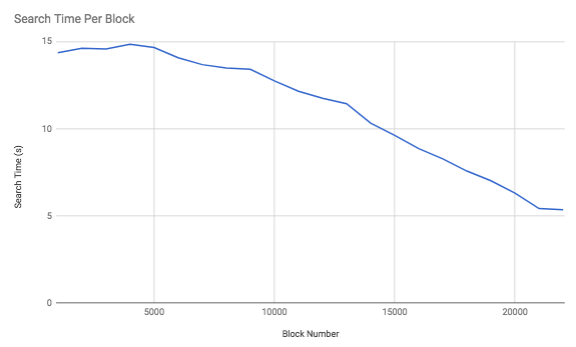
\includegraphics[width=0.9\columnwidth]{figures/draft-blocks.png}
 \caption{TODO
 \label{fig:opt}}
\end{figure}


\subsection*{Exp 5. Scaling}
\textbf{Sk. we exploit parallelism. This shows the stock dataset.}

\begin{table}[ht]
\centering
\label{my-label}
\begin{tabular}{|r|r|r|r|r|}
\hline
No Cores.   & No Cache & Cache Only & All Optimizations \\
\hline
1  & 4432.1   & 432.1      & 432.1             \\
\hline
2  & 2287.23  & 321.23     & 287.23            \\
\hline
4  & 1475.4   & 245.4      & 175.4             \\
\hline
8  & 806.7    & 206.7      & 106.7             \\
\hline
16 & 588.9    & 188.9      & 88.9              \\
\hline
32 & 378.4    & 162.4      & 78.4              \\
\hline
64 & 217.3    & 137.3      & 67.3    \\
\hline
\end{tabular}
\end{table}